\documentclass[3p]{elsarticle}

\usepackage{lineno,hyperref}
\usepackage{graphicx}
\usepackage{caption}
\usepackage{algorithm}% http://ctan.org/pkg/algorithms
\usepackage{algpseudocode}% http://ctan.org/pkg/algorithmicx
\usepackage{amsmath}

\modulolinenumbers[5]

\journal{Journal of Cryptography}

%%%%%%%%%%%%%%%%%%%%%%%
%% Elsevier bibliography styles
%%%%%%%%%%%%%%%%%%%%%%%
%% To change the style, put a % in front of the second line of the current style and
%% remove the % from the second line of the style you would like to use.
%%%%%%%%%%%%%%%%%%%%%%%

%% Numbered
%\bibliographystyle{model1-num-names}

%% Numbered without titles
%\bibliographystyle{model1a-num-names}

%% Harvard
%\bibliographystyle{model2-names.bst}\biboptions{authoryear}

%% Vancouver numbered
%\usepackage{numcompress}\bibliographystyle{model3-num-names}

%% Vancouver name/year
%\usepackage{numcompress}\bibliographystyle{model4-names}\biboptions{authoryear}

%% APA style
%\bibliographystyle{model5-names}\biboptions{authoryear}

%% AMA style
%\usepackage{numcompress}\bibliographystyle{model6-num-names}

%% `Elsevier LaTeX' style
\bibliographystyle{elsarticle-num}
%%%%%%%%%%%%%%%%%%%%%%%

\begin{document}

\begin{frontmatter}

\title{An Efficient Indexing Technique for AES Lookup Table to prevent Side-Channel Cache-Timing Attack}
%\tnotetext[mytitlenote]{Fully documented templates are available in the elsarticle package on \href{http://www.ctan.org/tex-archive/macros/latex/contrib/elsarticle}{CTAN}.}

%% Group authors per affiliation:
%\author{Elsevier\fnref{myfootnote}}
%\address{Radarweg 29, Amsterdam}
%\fntext[myfootnote]{Since 1880.}

%% or include affiliations in footnotes:
%\author[mymainaddress]{Refazul Islam Refat}
%\ead{refazul.refat@gmail.com}

%\author[mymainaddress]{Euna Islam}
%\cortext[mycorrespondingauthor]{Corresponding author}
%\ead{euna.islam@gmail.com}

%\author[mymainaddress]{Md. Mosaddek Khan $~^{*}$}
%\cortext[mycorrespondingauthor]{Corresponding author}
%\ead{mosaddek@cse.univdhaka.edu}

%\address[mymainaddress]{Computer Science and Engineering Department, University of Dhaka}
%\address[mysecondaryaddress]{360 Park Avenue South, New York}


\author[label1]{Refazul Islam Refat}\ead{refazul.refat@gmail.com}
 \author[label1]{Euna Islam}\ead{euna.islam@gmail.com}
 \author[label1]{Md. Mosaddek Khan\corref{*}}\ead{mosaddek@cse.univdhaka.edu}


 \address[label1]{Department of Computer Science and Engineering, University of Dhaka, Bangladesh}
% \address[label4]{Faculty of Engineering and Information Technology, University of Technology Sydney}
 %\address[label4]{Department of Computer Engineering, Kyung Hee University, South Korea}
  %\address[label5]{School of Computing and Mathematics, Charles Sturt University, Australia}

\cortext[*]{Corresponding Author. Mob.: 011900}

\begin{abstract}
In the era of virtualization, co-residency with unknown neighbours is a necessary evil and leakage of information through side-channels is an inevitable fact. Preventing this leakage of information through side-channels, yet maintaining high efficiency, has become one of the most challenging parts of any implementation of the Advanced Encryption Standard (AES) that is based on the Rijndael Cipher. Exploiting the associative nature of the cache and susceptible memory access pattern, AES is proved to be vulnerable to side-channel cache-timing attacks. The reason of this vulnerability is primarily ascribed to  the existence of correlation between the index Bytes of the State matrix and corresponding accessed memory blocks. In this paper, we idealized the model of cache-timing attack and proposed a way of breaking this correlation through the implementation of a Random Address Translator (RAT). The simplicity of the design architecture of RAT can make itself a wonderful choice as a way of indexing the lookup tables for the implementers of the AES seeking resistance against side-channel cache-timing attacks.
\end{abstract}

\begin{keyword}
AES\sep Cache-Timing Attack\sep Security
\end{keyword}

\end{frontmatter}

\linenumbers

\section{Introduction}

Out of the five candidate algorithms (MARS \cite{mars1998proposal}, RC6, Rijndael \cite{rijndael1998proposal}, Serpent \cite{serpent1998proposal}, and Twofish \cite{twofish1998proposal}) for the AES, Rijndael was pronounced as a new standard on November 26, 2001 as FIPS PUB 197 \cite{fips}. The security barrier of Rijndael cipher is so strong that a cryptographic break is infeasible with current technology. Even Bruce Schneier, a developer of the competing algorithm Twofish, admired Rijndael cipher in his writing, ``I do not believe that anyone will ever discover an attack that will allow someone to read Rijndael traffic" \cite{admire}.\\

A brute force method would require $2^{128}$ operations for the full recovery of an AES-128 key. A machine that can perform 8.2 quadrillion calculations per second will take 1.3 quadrillion years to recover this key. However, partial information leaked by side-channels can tear down down this complexity to a very reasonable level. Side-channel attacks do not attack the underlying cipher; they rather attack implementations of the cipher on systems that inadvertently leak data. Ongoing research in the last decade has shown that the information transmitted via side-channels, such as execution time \cite{spadavecchia2006network}, computational faults \cite{boneh}, power consumption \cite{kocher} and electromagnetic emissions \cite{em, em2, scards}, can be detrimental to the security of Rijndael \cite{daemen2002design} and other popular ciphers like RSA \cite{mit}.\\

We will be primarily focusing on the vulnerability of Rijndael AES to side-channel cache-timing attack and see how simple cache misses in a multiprogramming environment can lead to disastrous consequences. If the plaintext is known, recovery of half of the key by any privileged process is a matter of seconds. The prevention is not trivial; there exists trade-off between performance and degree of multiprogramming. We will present a concept that might balance this trade-off by introducing a little memory overhead. The biggest advantage could be that even though the process is arbitrary, the cipher text will always remain the same.\\

\section{Related Works}

In October 2005, Dag Arne Osvik, Adi Shamir and Eran Tromer presented a paper demonstrating several cache-timing attacks against AES \cite{osvikold}. One attack was able to obtain an entire AES key after only 800 operations triggering encryptions, in a total of 65 milliseconds. The attack required the attacker to be able to run programs on the same system or platform that is performing AES. That paper presented some decent defence against side-channel cache-timing attacks such as avoiding memory access, disabling cache sharing, dynamic table storage etc.\\

They revised their paper on 2010 \cite{osvik} and focused on modern microprocessor implementations and presented few more preventions. Most of them lacked conceptual consolidation and provided as implicit implication. Some of them even requires alteration of cipher text that might cause significant overhead in distributed systems to maintain synchronization. Other works included introduction of asynchronous circuitry in AES implementation \cite{spadavecchia2006network}.\\


\section{Preliminaries}

Before understanding the weakest part of the cipher, a clarified concept of cache memory and how they are accessed during real time AES implementation might be helpful.\\

\subsection{Memory Access in AES Implementations}

The memory access patterns of AES are particularly susceptible to cryptanalysis. The cipher is abstractly defined by algebraic operations and could, in principle, be directly implemented using just logical and arithmetic operations. However, performance-oriented software implementations on 32-bit (or higher) processors typically use an alternative formulation based on lookup tables as prescribed in the Rijndael Specification \citep{daemen2002design}.\\

Several lookup tables are precomputed once by the programmer or during system initialization. There are 8 such tables, $T_0,T_1,T_2,T_3$ and $T_0^{10},T_1^{10},T_2^{10},T_3^{10}$, each containing 256 4-byte words. The contents of the tables, defined in \citep{daemen2002design}, are inconsequential to most of the cache-timing attacks because of memory protection.\\

During key setup, a given 16-byte secret key $k=(k_0,k_1,...,k_{15})$ is expanded into 10 round keys, $K^{(r)}$ for $r=1,2,...,10$. Each round is divided into 4 words of 4 bytes each: $K^{(r)}=(K_0^{(r)},K_1^{(r)},K_2^{(r)},K_3^{(r)})$. The 0th round key is just the raw key: $K_j^{(0)}=(k_{4j},k_{4j+1},k_{4j+2},k_{4j+3})$ for $j=0,1,2,3$. The details of the rest of the key expansions are mostly inconsequential \citep{osvik}.\\

Given a 16-byte plaintext $p=(p_0,p_1,...,p_{15})$, encryption proceeds by computing a 16-byte intermediate state $x^{(r)}=(x_0^{(r)},x_1^{(r)},...,x_{15}^{(r)})$ at each round r. The inital state $x^{(0)}$ is computed by $x_i^{(0)}=p_i \oplus k_i ( i=0,1,...,15 )$.

\begin{center}
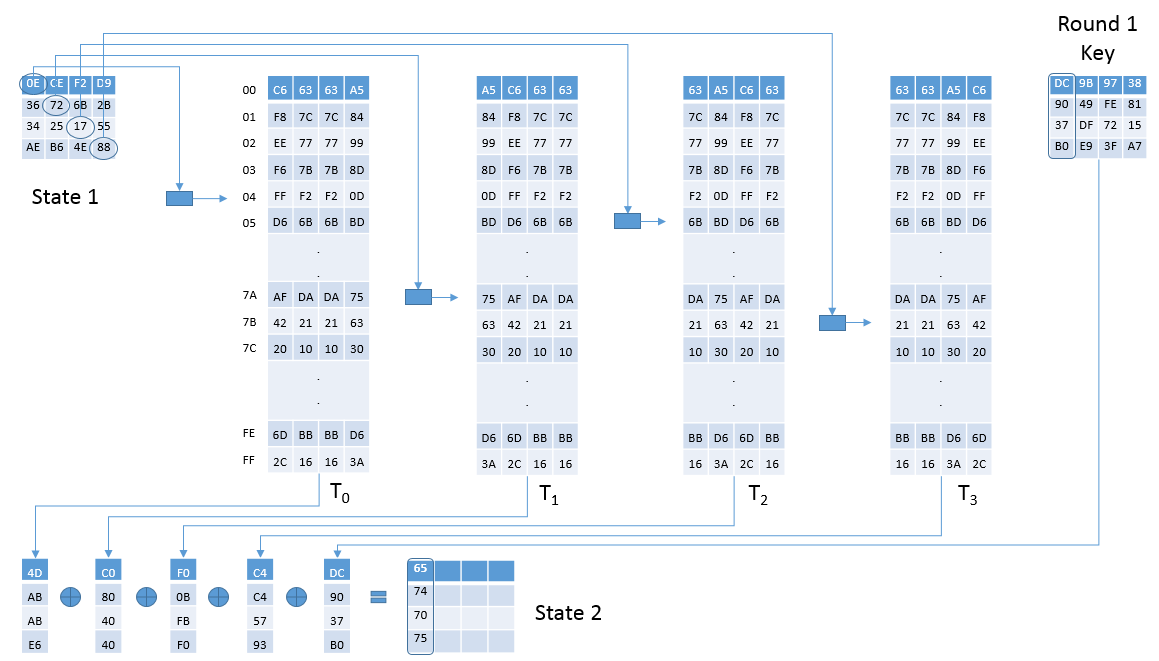
\includegraphics[scale=0.4,natwidth=1159,natheight=661]{Figures/aes-1-1(new).png}
\captionof{figure}{The figure demonstrates how $x_0^1,x_1^1,x_2^1,x_3^1$ are computed. Note that the bytes of the state matrix are being used as index of the lookup tables. Since the lookup table remains the same for a particular S-Box, an index byte will always cause lookup from the same block of cache memory}
\label{fig: The diagram shows how $x_0^1,x_1^1,x_2^1,x_3^1$ are computed.}
\end{center}

\begin{flushleft}
Thus, the first 9 rounds are computed by updating the intermediate state as follows, for $r=0,1,..,8$:
\end{flushleft}
\begin{small}
\begin{align*}
&(x_0^{(r+1)},x_1^{(r+1)},x_2^{(r+1)},x_3^{(r+1)}) \gets T_0[x_0{(r)}] \oplus T_1[x_5{(r)}] \oplus T_2[x_{10}{(r)}] \oplus T_3[x_{15}{(r)}] \oplus K_0^{(r+1)}\\
&(x_4^{(r+1)},x_5^{(r+1)},x_6^{(r+1)},x_7^{(r+1)}) \gets T_0[x_4{(r)}] \oplus T_1[x_9{(r)}] \oplus T_2[x_{14}{(r)}] \oplus T_3[x_{3}{(r)}] \oplus K_0^{(r+1)}\\
&(x_8^{(r+1)},x_9^{(r+1)},x_{10}^{(r+1)},x_{11}^{(r+1)}) \gets T_0[x_8{(r)}] \oplus T_1[x_{13}{(r)}] \oplus T_2[x_{2}{(r)}] \oplus T_3[x_{7}{(r)}] \oplus K_0^{(r+1)}\\
&(x_{12}^{(r+1)},x_{13}^{(r+1)},x_{14}^{(r+1)},x_{15}^{(r+1)}) \gets T_0[x_{12}{(r)}] \oplus T_1[x_1{(r)}] \oplus T_2[x_{6}{(r)}] \oplus T_3[x_{11}{(r)}] \oplus K_0^{(r+1)}
\end{align*}
\end{small}

Finally, to compute the last round, the above process of table-lookup is repeated with $r=9$, except that $T_0,T_1,T_2,T_3$ are replaced by $T_0^{(10)},T_1^{(10)},T_2^{(10)},T_3^{(10)}$. The resulting $x^{(10)}$ is the ciphertext. Compared to the algebraic formulation of AES, here the lookup tables represent the combination of \emph{ShiftRows}, \emph{MixColumns} and \emph{SubBytes} operations; the change of lookup tables in the last round is due to the absence of \emph{MixColumns} \citep{osvik}. It is clear from the above discussion that computation of a state matrix requires 16 Table lookups and 16 XOR operations.\\

We know, the first round state matrix is computed by XOR operation between the 16-byte plain text and the 16 byte plain key. One important point to notice from the previous discussion is that the state bytes are being used as index to the Lookup tables. Thus any Information of the accessed index will directly translate to Encryption Key Byte. For example, lets say we know $x_i^{(0)}$. Since plaintext is known for triggered encryptions, we know $x_i^{(0)}$ too.\\

\begin{align*}
x_i^{(0)} \gets x_i^{(0)} \oplus k_i^{(0)}
\end{align*}


\begin{center}
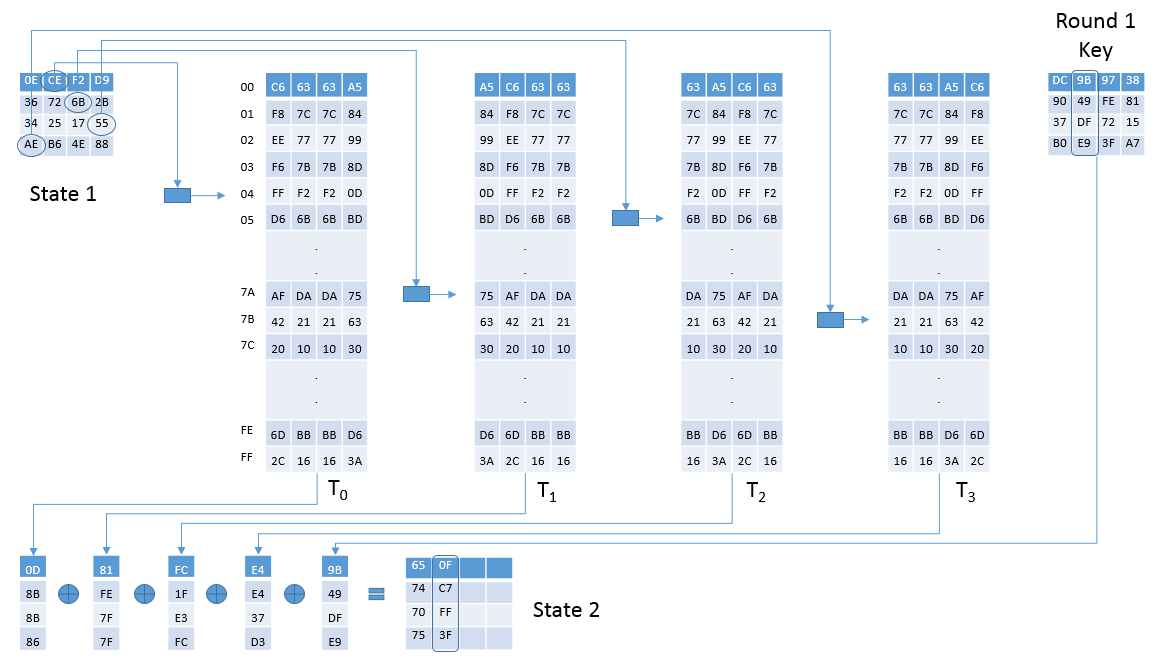
\includegraphics[scale=0.4,natwidth=918,natheight=525]{Figures/aes-1-2(new).png}
\captionof{figure}{The figure demonstrates how $x_4^1,x_5^1,x_6^1,x_7^1$ are computed.}
\label{fig: The diagram shows how $x_4^1,x_5^1,x_6^1,x_7^1$ are computed.}
\end{center}


%\begin{center}
%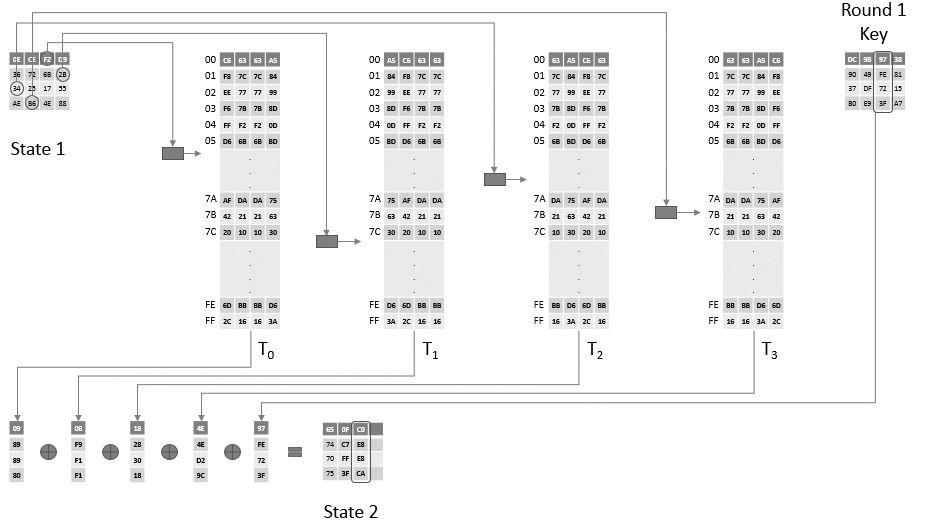
\includegraphics[scale=0.30,natwidth=925,natheight=521]{Figures/aes-1-3.png}
%\captionof{figure}{The diagram shows how $x_8^1,x_9^1,x_{10}^1,x_{11}^1$ are computed}
%\label{fig: The diagram shows how $x_8^1,x_9^1,x_{10}^1,x_{11}^1$ are computed.}

%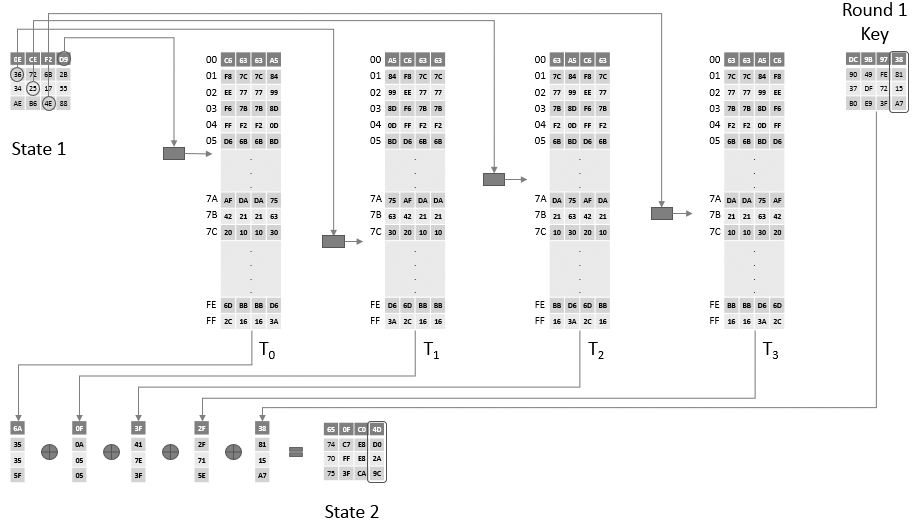
\includegraphics[scale=0.30,natwidth=917,natheight=521]{Figures/aes-1-4.png}
%\captionof{figure}{The diagram shows how $x_{12}^1,x_{13}^1,x_{14}^1,x_{15}^1$ are computed.}
%\label{fig: The diagram shows how $x_{12}^1,x_{13}^1,x_{14}^1,x_{15}^1$ are computed.}
%\end{center}

\begin{flushleft}
This implies,
\end{flushleft}
\begin{align*}
k_i^{(0)} \gets x_i^{(0)} \oplus x_i^{(1)}
\end{align*}

\begin{flushleft}
Thus knowing $x_i^1{(1)}$ for $i=0,1,2,...,15$ is sufficient to recover the full encryption key under the assumption that the plaintext is known. This is the weakest part of Round 1; in fact the weakest part of the Cipher.
\end{flushleft}

\subsection{How Lookup Tables fit in Memory and Cache}

Lets turn our attention to how AES Lookup tables fit in Memory and in Cache. We know, each Lookup table has 256 4-Byte entry. That gives it a total size of $256 \cdot 4=1024$ Bytes. Now, typical size of \emph{memory block} is 64 Bytes even on modern microprocessors. So for simplicity, we will assume the \emph{memory block} size $B$ to be 64 Bytes throughout this paper. Therefore, each table $T_i$ will occupy 16 memory blocks.

\begin{flushleft}
Also assume that, the initial address of $T_i$ congruent to the cache. That is, 1st block of the table will be cached in one of the $W$ \emph{cache lines} in the 1st \emph{cache set}.
\end{flushleft}

\section{The Idealized Prime+Probe Technique}

The Prime+Probe technique helps to visualize the vulnerability of AES Cipher during the 1st Round. To keep things simple, we'll consider an idealized environment in which only the attacking process and the victim encrypting process exists. Also assume that the attacking process will be able to invoke or interrupt the encrypting process at any time. Now since we are talking about triggered encryption, the plaintext is always known.

\begin{center}
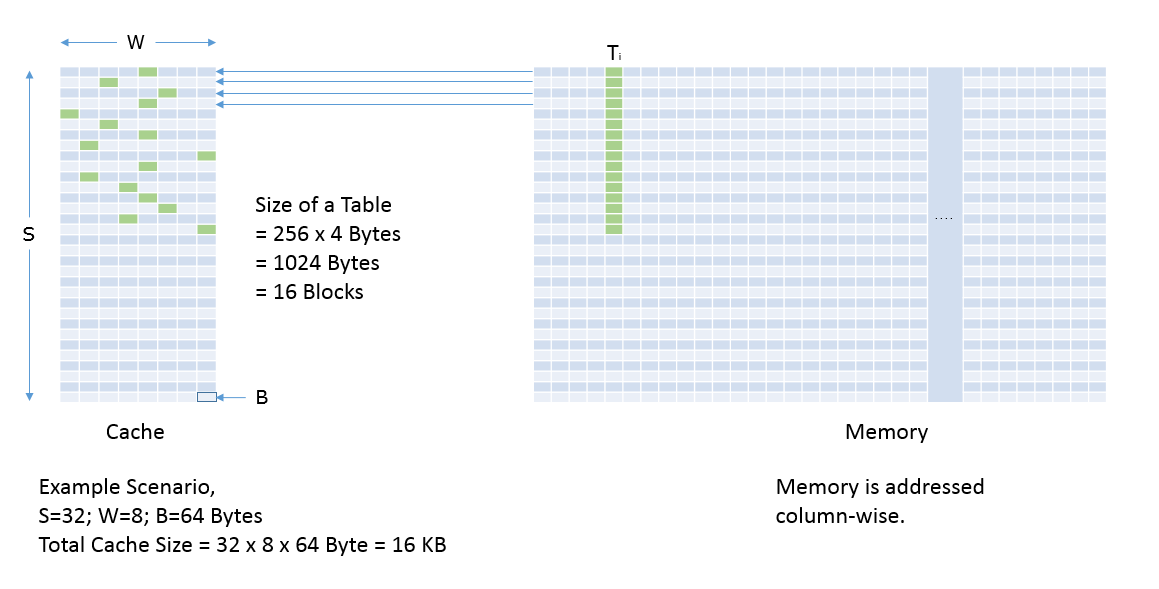
\includegraphics[scale=0.4,natwidth=1159,natheight=589]{Figures/lookup(new).png}
\captionof{figure}{Demonstration of how AES Lookup Table fits in memory and cache. On the left side, number of rows implies total number of cache sets, whereas, number of columns implies associativity of the cache. On the right side, instead of depicting memory as a continuous array of blocks, it is portrayed in congruence with cache memory. Note that all blocks in a row of memory competes for the blocks of corresponding row in cache memory. }
\label{fig: Demonstration of how AES Lookup Table fits in memory and cache.}
\end{center}

\begin{flushleft}
The Prime+Probe technique has the following 3 phases:
\end{flushleft}

\begin{itemize}
\item Prime
\item Trigger
\item Probe
\end{itemize}

\paragraph{Prime}
During the Prime phase, the Cache is filled completely by the attacking process. This can be done by allocating a contiguous amount of memory as big as the size of the cache and performing a read on it. If $S=32$, $W=8$ and $B=64$ Bytes, then

\begin{center}
Total size of the cache $=S\cdot W \cdot B=16$ KB
\end{center}

As implied by the figure above, performing a serial read on a contiguous memory as big as the cache results in inception of filling the cache. Continuing this way, we'll end up filling the cache completely after the reading is finished.

\paragraph{Trigger}
With the Cache filled with our data, we're in a position to invoke the encrypting process and trigger an encryption of some known plain text. As the encrypting process reaches the First Round and performs the first lookup, it is interrupted. An important point to note here is, we're idealizing the model to illustrate the susceptibility of the First Round. Recovering the AES Encryption Key is not the actual intent of this paper.

\begin{center}
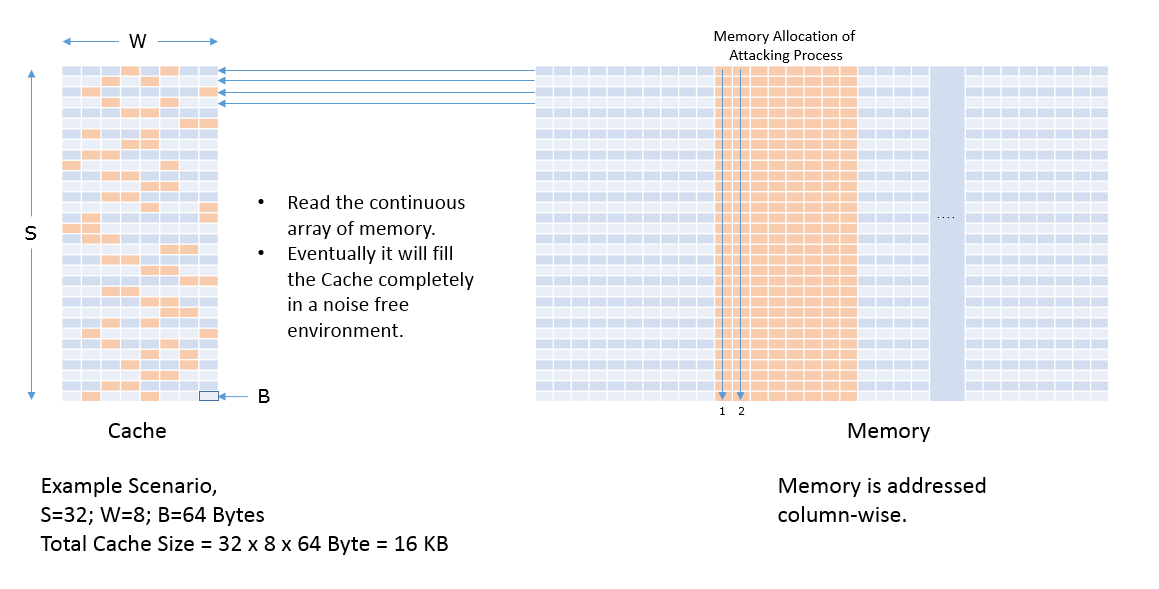
\includegraphics[scale=0.4,natwidth=1159,natheight=589]{Figures/filling(new).png}
\captionof{figure}{Demonstration of the Cache filling process. Note that reading continuous array of memory will cause allocation of one block from each cache set and due to Principle of Locality, immediate next read cycle will cause allocation of another block (different from the previous) from each cache set.}
\label{fig: Demonstration of the Cache filling process.}
\end{center}


\paragraph{Probe}
After we interrupt the encrypting process just after it performed its first lookup during the First Round of AES, we perform the Prime again, i.e. we fill the cache again. But this time, we maintain a clock measuring of how long it takes to read a \emph{memory block}. Before the Trigger phase, the cache was completely filled by our data. But after that Trigger phase, one block of the 
Lookup table $T_0$ is now in the cache due to the lookup operation. So all but that block will suffer from a cache miss.

\begin{center}
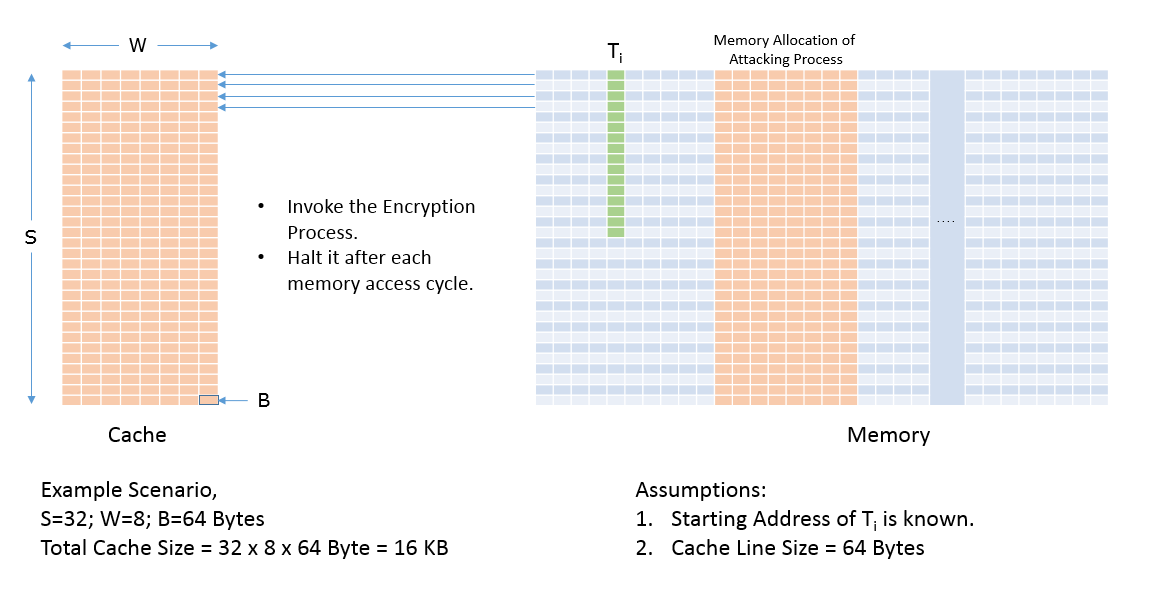
\includegraphics[scale=0.4,natwidth=1159,natheight=589]{Figures/prime(new).png}
\captionof{figure}{Demonstration of the Prime phase where reading a continuous array of memory equal to the size of the cache will eventually fill the cache completely with attacker's data in a noiseless environment.}
\label{fig: Demonstration of the Prime phase.}
\end{center}

Observing the position of the cache miss, we can easily identify which block of $T_0$ was accessed since we assumed Lookup Tables $T_i$ to be congruent with the cache. Now if we can identify which block of $T_0$ was accessed during the First Round, we can extract some valuable piece of information. Since size of \emph{memory block} is 64 Bytes, each \emph{memory block} holds 16 entry of the Lookup Table. So for example, if 7th block of $T_0$ was accessed, we can conclude the index $x_0^{(1)}$ was somewhat between 0x60 and 0x6F, i.e. high nibble is 0x6. We know

\begin{align*}
x_0^{(1)}=x_0^{(0)} \oplus k_0^{(0)}
\end{align*}

\begin{center}
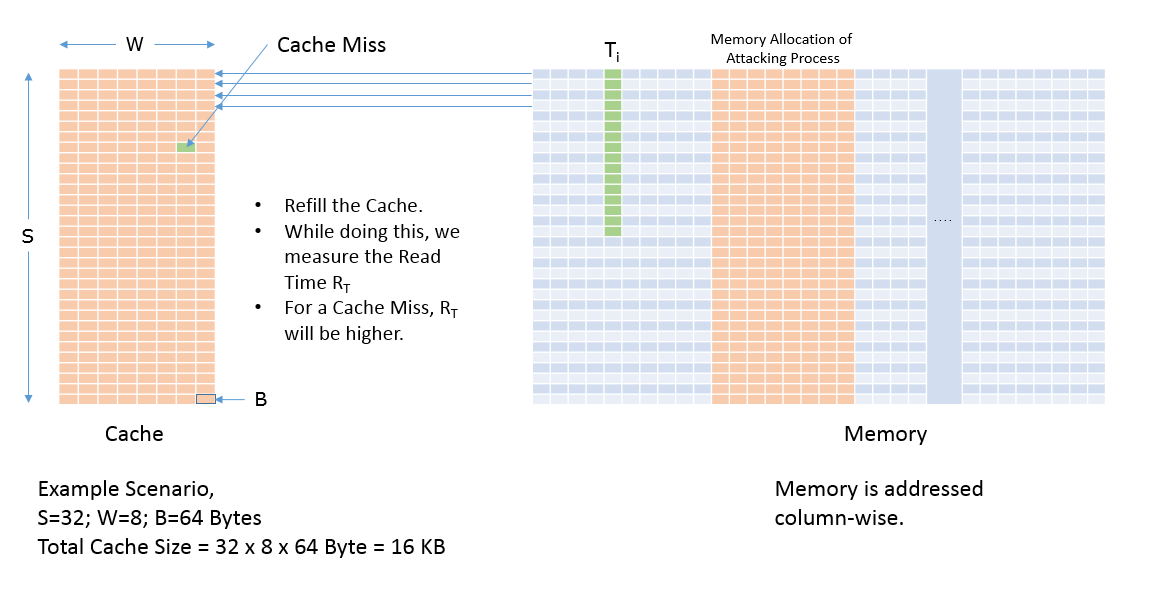
\includegraphics[scale=0.4,natwidth=1159,natheight=589]{Figures/probe(new).png}
\captionof{figure}{Demonstration of how information about the location of the cache miss during first round reveals critical information about the encryption key. In the example scenario, the high nibble of a Byte (0x6) is easily gleaned.}
\label{fig: Demonstration of the Probe phase.}
\end{center}

Here $x_0^{(0)}$ is the 1st Byte of the plaintext and $k_0^{(0)}$ is the 1st Byte of the Encryption Key. Now, since addition and subtraction in Galois Field are the same XOR operation, rearranging the equation yields:
\begin{align*}
k_0^{(0)}=x_0^{(0)} \oplus x_0^{(1)}
\end{align*}

Because we know $x_0^{(0)}$ from the plain text and the high nibble of $x_0^{(1)}$ from the Prime+Probe technique, we can compute the high nibble of the first Byte of the Encryption Key by a simple XOR operation. Proceeding this way for every Bytes $x_i^{(1)}$ for $i=0,1,2,...,15$, we can calculate $k_i^{(0)}$ for $i=0,1,2,...,15$ and dig up half of the Encryption Key. The idealized procedure is summarized in algorithm 1.

\begin{algorithm}
\caption{Abstract procedure for capturing half of the Key during the First Round}
\label{Abstract procedure for capturing half of the Key during the First Round}
\begin{algorithmic}[1]
	\State triggerEncryption()
	\For{$i \gets 0$ to $15$}
		\State fillCache()
		\State haltEncryption()
		\State $j \gets$ missedBlockIndex()
		\State $j \gets j\ll 4$
		\State $k_i^{(0)} \gets j \oplus x_i^{(0)}$\Comment{$k_i^{(0)}$ and $x_i^{(0)}$ resemble i-th Byte of the key and known plaintext respectively}
	\EndFor
\end{algorithmic}
\end{algorithm}

\section{Proposed Random Address Translator (RAT)}

From the analysis in the previous sections, it is prominent that the existence of linear correlation between index Bytes of the state matrix and the location of corresponding accessed block in memory is the primary reason of vulnerability of AES in the first round. Given size of memory block (64 Bytes in most of the cases), any information about the memory access during the encryption process would directly reveal high nibble of the index Bytes. Thus if the size of the key is 128 Bit, pre-knowledge of the high nibbles of the index Bytes would reduce the brute force complexity to $2^{64}$. A machine that can perform 1 quadrillion operations per seconds would take less than 5 seconds to break the rest of the key in brute force attempt.\\

If the correlation can be broken, so that the index Byte will no longer be used directly to locate the desired block of the Lookup table, most of the cache-timing threats will be eliminated. The key concept to the solution is to perform memory access to get the desired content from an arbitrary, unpredictable location. This can be accomplished by introducing a Translator table between the state matrix and the Lookup table.

\begin{center}
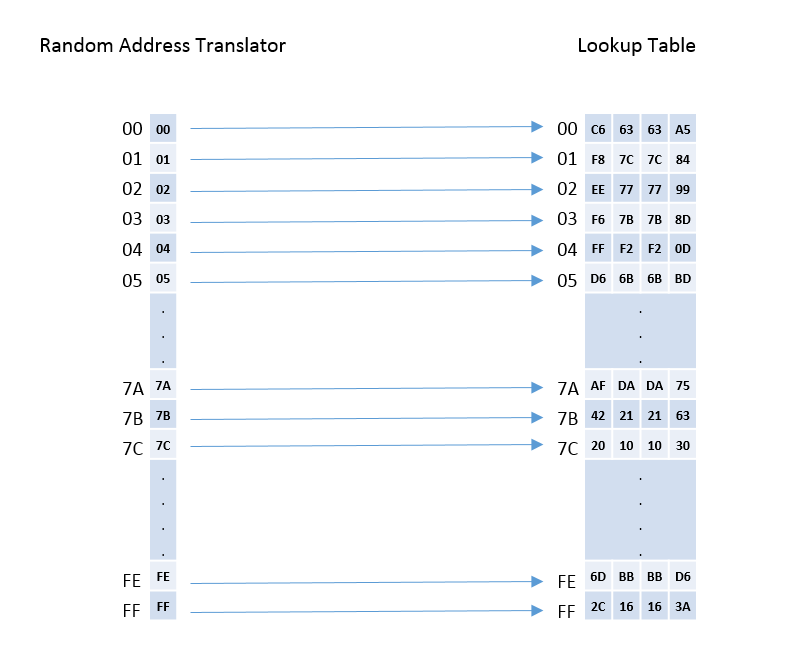
\includegraphics[scale=0.4,natwidth=785,natheight=666]{Figures/rat-init(new).png}
\captionof{figure}{Random Address Translator Initialization.}
\label{fig: Random Address Translator Initialization.}
\end{center}

The Translator table is initially aligned with the Lookup table as illustrated in figure 7. This implies that if the address of $i$-th row in the lookup table is $X_i$, the content of the $i$-th row of the Translator table is also $X_i$. So initially it has no effect on the accessed memory block of the lookup table because it is fully aligned with it. After that, lets take two rows of the Translator table $T_i$ and $T_j$ and corresponding two rows of the original lookup table $L_i$ and $L_j$ and perform a swap between them. This is illustrated in figure 8.

\begin{center}
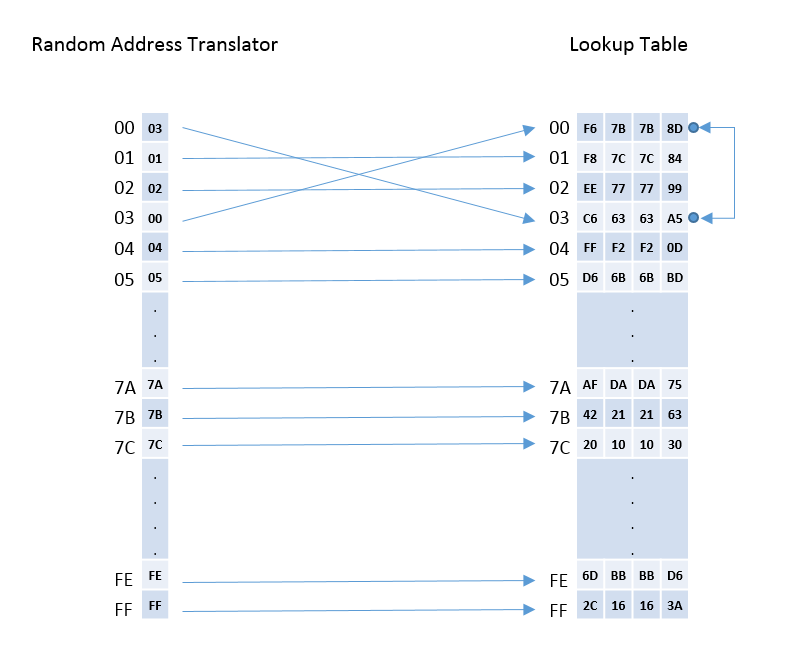
\includegraphics[scale=0.38,natwidth=785,natheight=666]{Figures/rat-step-1.png}
\captionof{figure}{Random Address Translator after first swap.}
\label{fig: Random Address Translator after first swap.}
\end{center}

Continuing this way, there can be at most 128 swaps between the entries of the table. Note that an entry can be swapped only once, so keeping trace of swapped entries is important. After scrambling, the correlation is completely broken as illustrated in figure 9.

\begin{center}
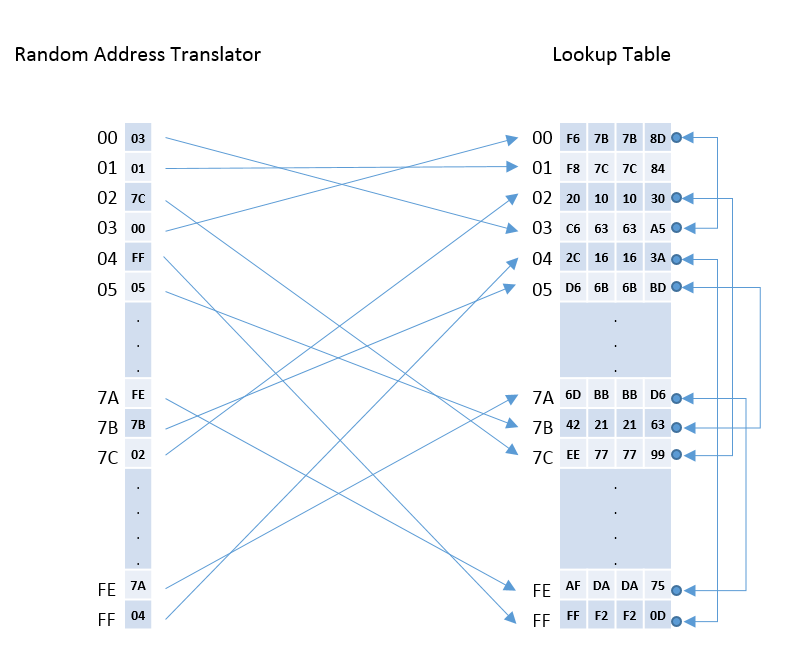
\includegraphics[scale=0.38,natwidth=785,natheight=666]{Figures/rat-scrambled(new).png}
\captionof{figure}{Random Address Translator completely scrambled. It can be noticed that some of the entries can be left ``unswapped'' as the process is arbitrary. Here 2nd entry is left intact.}
\label{fig: Random Address Translator Scrambled.}
\end{center}

With the RAT activated, there is no such phrase such as, index 0x05 will access the 1st block of the Lookup table. Because the content of the address 0x05 is now at 0x7B address (from the figure above) and that tracing is recorded by the RAT. The procedure for constructing the RAT is formulated in algorithm 2 and 3.

\begin{algorithm}
	\caption{Constructing the RAT}
	\label{Constructing the RAT}

	\begin{algorithmic}[1]
	
	\Function{init}{\null}
	\State $x\gets \{0,1,2,....,15\}$
	\State $y\gets \{0,1,2,....,15\}$
	\State $rat\gets\{0,0,0,0\}$
	\For{Arbitrary number of times}
		\State $i\gets rand() \bmod 16$\Comment{$\bmod$ resembles modulus operation}
		\State $j\gets rand() \bmod 16$
		\State $swap(x_i,x_j)$
		\State $y_{x_j}\gets i$
		\State $y_{x_i}\gets j$
	\EndFor
	\For{$i\gets0$ to $7$}
		\State $rat_0 \gets rat_0 + x_i\ll((7-i)\ll2)$\Comment{$\ll$ resemebles bitwise left shift operation}
		\State $rat_1 \gets rat_1 + x_{i+8}\ll((7-i)\ll2)$
		\State $rat_2 \gets rat_2 + y_i\ll((7-i)\ll2)$
		\State $rat_3 \gets rat_3 + y_{i+8}\ll((7-i)\ll2)$
	\EndFor
	\State delete x,y
	\State return rat
	
	\EndFunction	
	\end{algorithmic}
\end{algorithm}

After that, a scrambling is done on both tables simultaneously and arbitrarily. Note that no entry is allowed to be scrambled or swapped with other entry more than once. Also note the presence of \emph{rand()} methods. It symbolizes the randomness of the swapping process.

\begin{algorithm}
	\caption{Mapping Fuction}
	\label{Mapping Function}

	\begin{algorithmic}[1]

	\Function{map}{i}
	\If{$((i \mathrel{\&} 128)=0)$}\Comment{$\mathrel{\&}$ resembles bitwise and operation}
		\State $j \gets 0$
	\EndIf
	\State $k \gets ((255-i)\gg 4)\ll 2$\Comment{$\ll$ and $\gg$ resemble bitwise left and right shift operations respectively}
	\State $x \gets (rat_j\gg k)\mathrel{\&} 15$
	\State $y \gets i \mathrel{\&} 15$
	\State return $(x\ll 4)+y$
	\EndFunction

	\end{algorithmic}
\end{algorithm}

\begin{algorithm}
	\caption{Mingling Function}
	\label{Mingling Function}

	\begin{algorithmic}[1]

	\Function{mingle}{table}\Comment{Takes unmodified lookup table as parameter}
	\For{$i \gets 0$ to $255$}
		\For{$j \gets 0$ to $3$}
			\State $temp_{i,j} \gets table_{map(i),j}$
		\EndFor
	\EndFor
	\For{$i \gets 0$ to $255$}
		\For{$j \gets 0$ to $3$}
			\State $table_{i,j} \gets temp_{i,j}$
		\EndFor
	\EndFor
	\State delete $temp$
	\State return $table$
	\EndFunction

	\end{algorithmic}
\end{algorithm}

\begin{algorithm}
	\caption{Inverse Mapping Fuction}
	\label{Inverse Mapping Function}

	\begin{algorithmic}[1]

	\Function{inverseMap}{i}
	\State $j \gets 3$
	\If{$((i \mathrel{\&} 128)=0)$}\Comment{$\mathrel{\&}$ resembles bitwise and operation}
		\State $j \gets 2$
	\EndIf
	\State $k \gets ((255-i)\gg 4)\ll 2$\Comment{$\ll$ and $\gg$ resemble bitwise left and right shift operations respectively}
	\State $x \gets (rat_j\gg k)\mathrel{\&} 15$
	\State $y \gets i \mathrel{\&} 15$
	\State return $(x\ll 4)+y$
	\EndFunction
	\end{algorithmic}
\end{algorithm}

\section{Performance Evaluation}

There are some other proposed solutions in this field \citep{osvik,paladi,rudra2001efficient,matsui2006far,matsui2007power,konighofer2008fast,meushaw2005device}. We take some of the most prominent ones and compare it with our proposed solution.\\

\paragraph{Avoiding Memory Access}
Since the cache-timing attacks exploit the effect of memory access on the cache, any implementation that does not perform any table lookup won't suffer from this sort of attacks. But this solution has a major drawback. The performance is degraded by an order of magnitude. The SubBytes Transformation phase requires 16 table lookups for the 16 Bytes of a State matrix. The ShiftRows Transformation phase requires 16 shift operations. The MixColumns Transformation phase requires 8 shift operations, 8 conditional XOR operations and 12 mandatory XOR operations. Finally the AddRoundKey Transformation phase requires 16 XOR operations.\\

To summarize the fact, we need a total of 24 shift operations, 16 table lookups, 8 conditional XOR operations, 28 mandatory XOR operations for a single round. This is demonstrated in figure 10.

\begin{center}
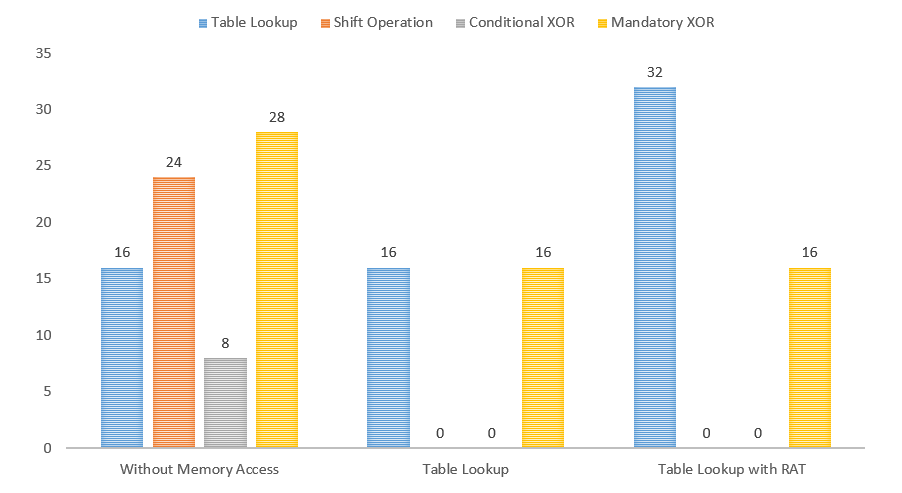
\includegraphics[scale=0.4,natwidth=902,natheight=493]{Figures/withnormal(new).png}
\captionof{figure}{Comparison of RAT with straightforward AES implementations in a single round. An implementation that completely avoids memory access requires 16 table lookups, 24 shift operations and 36 XOR operations (8 of which them are conditional), whereas introduction of RAT incurs 2 times more table lookups and 16 XOR operations in a single round.}
\label{fig: Comparison of RAT with Straightforward AES Implementation.}
\end{center}

In fact, the conditional XOR operation is vulnerable to timing attack too \citep{stallings5}. Other than lagging behind in terms of security, straightforward implementation required more computation time. So avoiding memory access doesn't save the day. But the positive side is, straightforward implementation doesn't need to maintain any sort of lookup table other than the S-Box. On the other hand table lookup with RAT has an overhead of maintaining two table. The Lookup table requires 4096 Bytes of memory space and RAT requires another 1024 Bytes of space.

\begin{center}
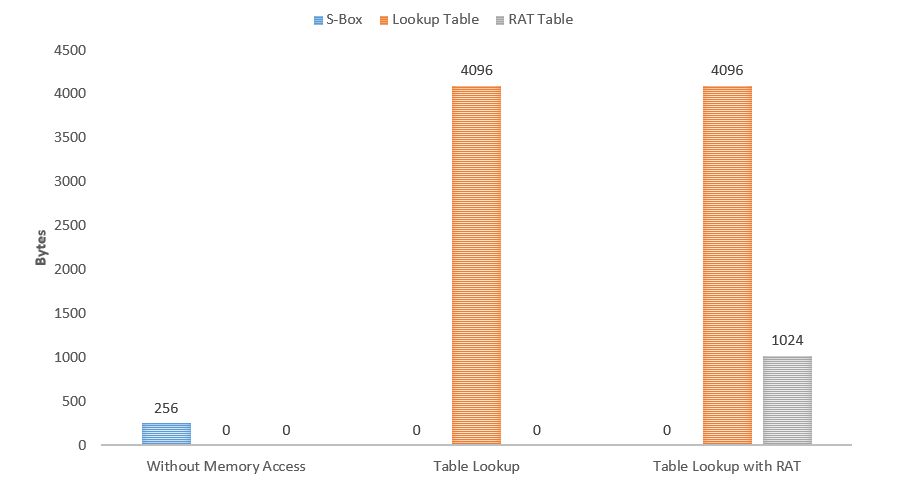
\includegraphics[scale=0.4,natwidth=902,natheight=493]{Figures/performance_memory(new).png}
\captionof{figure}{Performance Evaluation of RAT in terms of Memory Usage.}
\label{fig: Performance Evaluation of RAT in terms of Memory Usage.}
\end{center}

\paragraph{Disable Cache Sharing}
To protect against software-based attacks, it would suffice to prevent cache state effects from spanning process boundaries. But practically this is very expensive to achieve. On a single threaded processor, it would require flushing all caches during every context switch. On a processor with simultaneous multi threading, it would also require the logical processors to use separate logical caches, statically allocated within the physical cache; some modern processors do not support such a mode \citep{osvik}. Using RAT will not impose any restriction about cache sharing which is perfectly suitable for cloud environment and virtual machines (without causing evictions and filling).

\paragraph{Static or Disabled Cache}
One brutal countermeasure against the cache-base attacks is to completely disable the CPU's caching mechanism. Of course, the effect on performance would be devastating. A more attractive alternative is to activate a ``no-fill" mode where the memory accesses are serviced from the cache when they hit it, but accesses that miss the cache are serviced directly from the memory

\begin{enumerate}
\item Preload the AES tables into the cache
\item Activate the ``no-fill" mode
\item Perform encryption
\item Deactivating ``no-fill" mode
\end{enumerate}

The section spanning (1) and (2) is critical, and attacking process must not be allowed to run during this time \citep{osvik}. However, the major drawback of this approach is that, during the encryption process the overall system will be slowed down by a factor since cache access is limited during the encryption process. But using RAT, the ``no-fill" mode is not required. All the other processes can be allowed to access the cache even during the encryption proceeds.\\

\paragraph{Dynamic Table Storage}
The cache-based attacks observe memory access patterns to learn about the table lookups. Instead of eliminating these, we may try to decorrelate them. For example, one can use many copies of each table, placed at various offsets in memory, and have each table lookup use a pseudorandomly chosen table. Somewhat more compactly, one can use a single table, but pseudorandomly move it around memory several times during each encryption \citep{osvik}. But the major drawback of this approach is that, it will incur cache misses more than ever. This implies that the encryption process will be slowed down by a factor. More importantly the performance and security of this approach are very architecture dependent. Using RAT helps us alleviate this situation by obviating the need of moving around the Lookup table in the memory.

\subsection{Other Major Advantages}
Some important benefits of using the RAT are
\begin{itemize}
\item The Cipher Text remains the same and the AES implementation becomes a client dependent process. We don't need to worry about how other ends of the terminals are encrypting their data. As long as the key doesn't change, Cipher Text remains the same. 
\item No need of NOP operation. NOP operations are introduced to scramble uniform patterns in various fields. In case of cache-timing analysis, NOP operation would mean accessing Lookup table entry, but doing no operation with it.
\item No need to introduce disturbance in plaintext. Sometimes plaintext is modified before it is passed to the encrypting process. This sort of approach is not suitable for large scale application where the interface must be kept as simple as possible.

\end{itemize}

\section{Future Works}

\begin{itemize}

\item There are some limitations in the process of constructing the RAT table. One major limitation is that swapping is not allowed more than once for an entry. Thus there can be a maximum of 128 swaps for a single Lookup table. To allow more number of swaps per entry, more sophisticated data structure is required.

\item The big picture that summarises the performance difference with the straightforward Table lookup approach is given below

\begin{center}
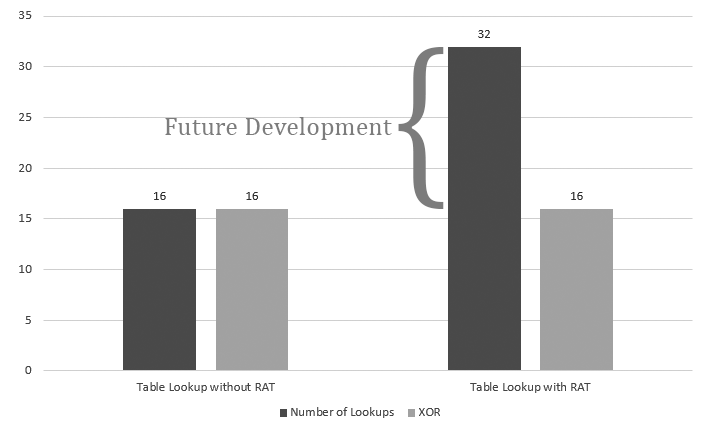
\includegraphics[scale=0.4,natwidth=713,natheight=436]{Figures/performance.png}
\captionof{figure}{Comparison with straightforward Table Lookup approach.}
\label{fig: Comparison with straightforward Table Lookup approach.}
\end{center}

As we can see, we need 2 times more table lookups than the ordinary approach. The area of future development is to reduce this factor.

\item Another big concern is that, RAT tables add a fair amount of memory overhead to the encrypting process. Whereas the Lookup tables altogether require 4KB of space, RAT tables requires 1KB of space. Although not a big figure to worry about, space overhead can be reduced with the assistance of some more tables of smaller sizes.

\end{itemize}

\section{Conclusion}

Side channel attacks don't divulge everything overnight; instead they ease the calculations and assumptions that helps rest of the operations accomplished in bounded time. Although the existing AES encryption model has sufficient complexity to blow away any straightforward attempt to break the security, side-channels still poses a real threat and a bad implementation of the cipher might lead to dire consequences.\\

The most challenging part of security is now making the implementation of the existing ciphers resistant to side-channel attacks. Preventing leakage of information through side-channel is not a trivial task at all. The experiment has shown that even the straightforward Table lookup approach can be made secure without the assistance of any piece of special software or hardware. And that might be the most important requirement in the industry.

\clearpage


\section*{References}

\bibliography{mybibfile}

\end{document}
